\chapter{Getting Ready to Get Tactical}

\centering
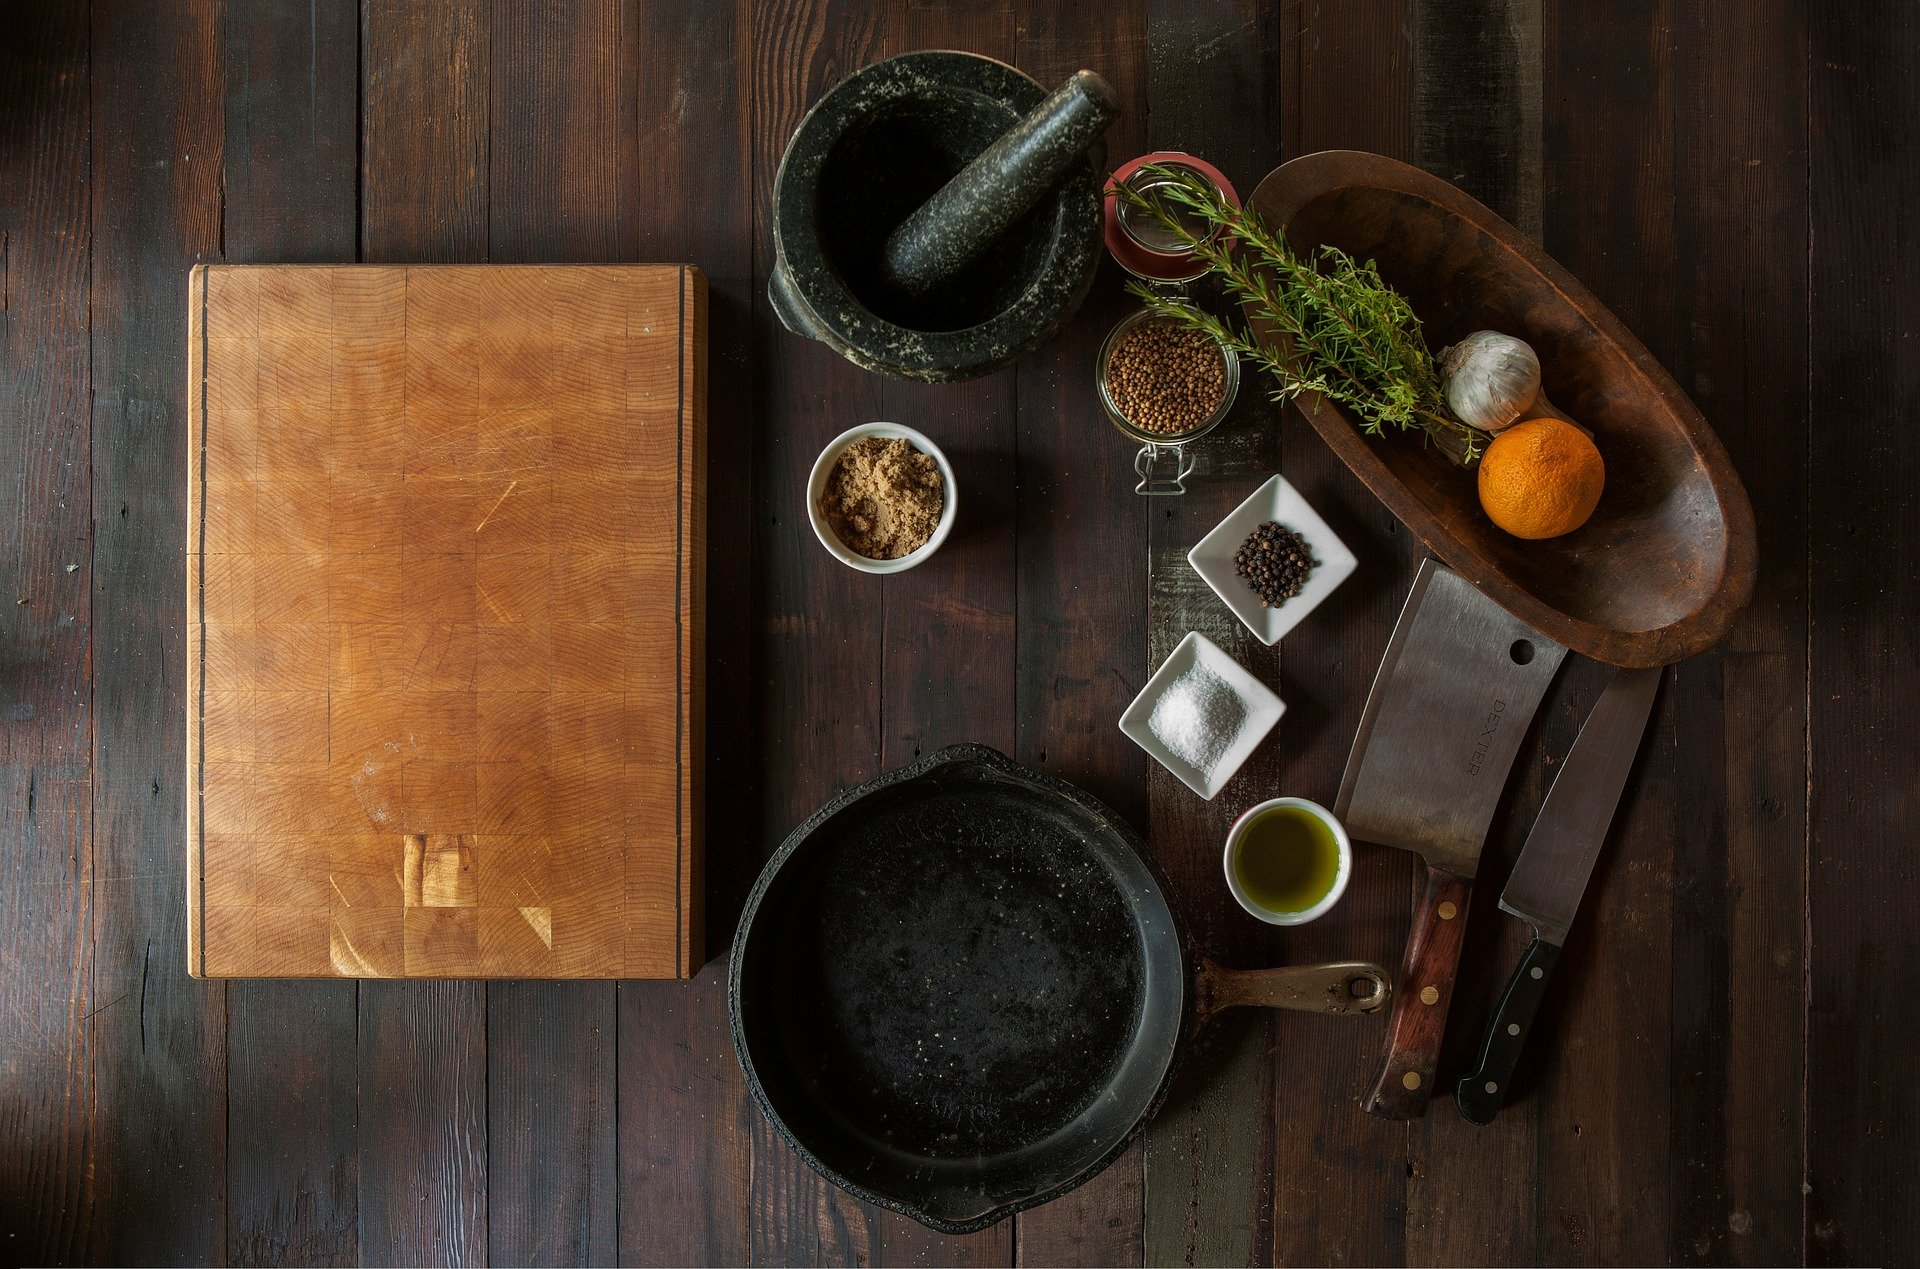
\includegraphics[scale=0.20]{images/ingredients-498199_1920.jpg}


\justify{}
Think of this chapter as the \emph{mise en place} of our DevSecOps souffle. We will increase our chances of success
by preparing our work environment for the project at hand. Let's start our preparations by outlining our
overall objectives. We want to:

\justify{}
\begin{itemize}
	\item
	      Create an extensible lab environment for rapid prototyping and development.
	\item
	      Keep our lab costs down while meeting the rest of the objectives.
	      Utilize free services and open source tools to the extent possible.
	\item
	      Use the published best practices for each tooling, operations, or
	      development ecosystem we choose to employ.
	\item
	      Always leave our projects in a functional state.
	\item
	      Get out of our old comfort zone, into a new one.
\end{itemize}

\section{Prerequisites}

\justify{}
This book intends to be a practical treatment of common and popular technologies from the DevSecOps world. As such, we assume
the reader has some basic knowledge of certain concepts. We will be exploring new ways of working for folks who
are somewhat familiar with:

\begin{itemize}
	\item
	    Linux (UI and command line)
	\item 
        Python 3
	\item
	    Familiarity with github.com and the concepts of pull requests and branching.
\end{itemize}

\justify{}
The examples in this book have been tested on Linux running the latest version of Docker. For more
intformation about installing Docker, see \href{https://docs.docker.com/get-docker/}{the Get Docker section}
of their website. There are directions there for installing Docker on Linux, Mac, and other operating systems.

Let's take a look at some of the other foundational environmental elements we need in place to be successful.

\section{Packages}

\subsection{MacOS}

Homebrew bills itself as \href{https://brew.sh/}{the missing package manager for MacOS}. Using ``brew'' and also
``cask'' to install and manage packages on MacOS will make your life much simpler.

\justify{}
It is also recommended that you familiarize yourself with the Terminal application on MacOS. Note that brew
commands are executed form within the terminal rather than using the GUI. Also bear in mind that packages are
installed with your user account. In other words, ``SuperUser'' privileges are not just discouraged, they are
neither required nor desired.

\subsection{Linux}

My prefered environment is a Debian based Linux distribution. Ubuntu, Cinnamon, and PopOS are all examples of 
Linux distrubutions in this family. While some code examples and lab containers use Debian-based distros, you
may also encounter Alpine Linux (typically chosen for it's smaller image size), amoung others.

\section{The Workhorse (IDE)}

\begin{figure}[!htb]
\centering
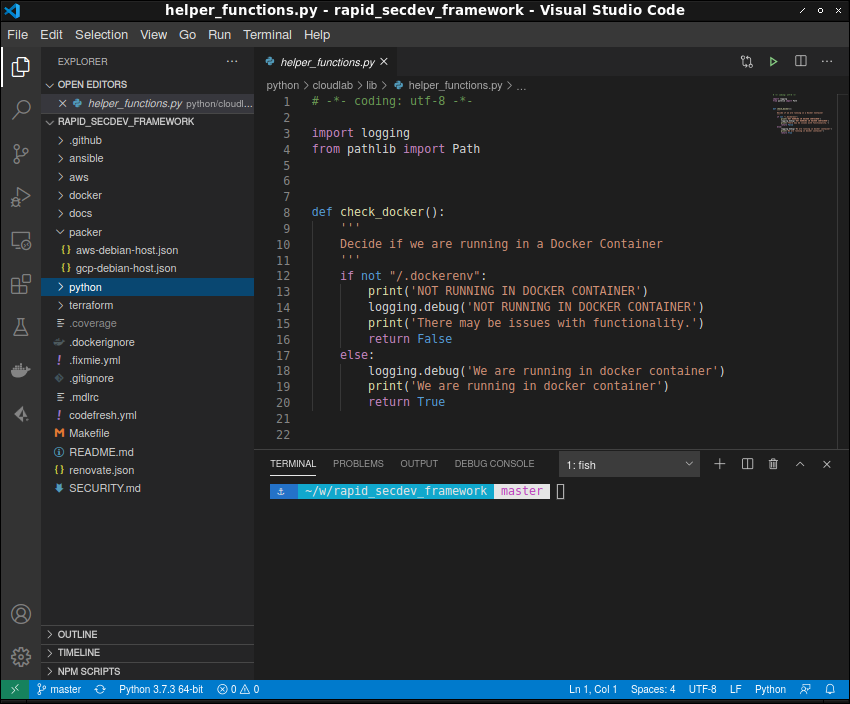
\includegraphics[scale=0.45]{images/setup-vscode.png}
\caption{The VScode IDE.}
\label{vscode-ide}
\end{figure}

\justify{}
It is quite helpful to have a piece of software on your workstation that makes code and document creation and edits easier. This
software is commonly known as an Integrated Development Environment (IDE)\index{IDE}. A decent IDE with the right add-ons can
provide syntax highlighting to show potential issues you might have missed, help you check for spelling or
grammar mistakes in your documentation, and even makes suggestions on alternate ways of writing your code.

\justify{}
There are many commercial and Open Source IDEs available. Visual Studio Code from Microsoft is a popular choice due to it's easy
installation. VSCode\index{VSCode} works well on Linux, Mac and other operating systems.
The environment is easily extensible to support most any language, linter, or syntax checker we may have a need
for, thanks to their easy to use and well integrated ``Extension'' feature. VSCode also has an integrated terminal
window\index{Terminal Window} so the developer can execute shell commands without leaving the IDE screen.

\section{SSH Key Setup}

\justify{}
Take note of the fact that setting up SSH keys means generating a pair of keys, not a single key. This is an important 
distinction. You will want to add your public key to sites like \href{github.com}{github.com}. The public key half will
also be added to machine instances that you create with public cloud providers. This will allow you to log in without
having to provision a user/password combination. You should take care to 
protect the private key at all times. Under no circumstances should you share your private SSH key.\cite{ssh}
\justify{}
Take a few minutes to generate an SSH key\index{SSH keys} pair if you don't already have one. We will add the public half of
our SSH key pair to hosts we provision. The directions for generating an SSH keypair found on the
\href{github.com}{github.com} website are perfect for our setup task. Follow the directions in the article 
\href{https://docs.github.com/en/github/authenticating-to-github/connecting-to-github-with-ssh/generating-a-new-ssh-key-and-adding-it-to-the-ssh-agent}{Generating a new SSH key and adding it to the ssh-agent}

\subsection{Generating a Key from the Command Line}

If you are using a Linux or Mac system, you have the option to create your SSH key pair from the command line. Consider 
the following example code listing.

\begin{mybox}{\thetcbcounter: SSH Key Generation}
\lstinputlisting{code/13-setup/ssh-key-generation}
\end{mybox}

\justify{}
Now you can add your public key half to your user settings in \href{github.com}{github.com}. For me it makes sense to have
two key pairs, one used for work projects, and one used for personal projects.

\section{GPG Key Setup}

\justify{}
\href{https://gnupg.org/}{Gnu Privacy Guard (GPG)} is an Open Source replacement for Symantec's PGP software. It allows you
to generate an asymmetric key pair that can be exchanged with other users, encrypt your personal files, or verify your identity.
Again, you will want to be sure to share your public key and protect your private key. This is the same reasoning we used in the
case of our SSH keys.

\justify{}
We will use a GPG key to sign commits to GitHub\index{GitHub}. This will help others verify that work you check in to revision
control did actually come from you. It's not strictly necessary but is considered good practice.
Some repositories require that you sign your pull requests with your GPG key\index{GPG key}.

\justify{}
Take a few minutes to set up a GPG key. Once you have an account setup, you can add
it to your profile on \href{github.com}{github.com}.

\subsection{Command Line GPG Key Setup}

\begin{mybox}{\thetcbcounter: Command Line GPG Key Setup}
\lstinputlisting{code/13-setup/gpg-key-setup}
\end{mybox}

\justify{}
Copy your GPG key, beginning with the string ``BEGIN PGP PUBLIC KEY BLOCK'' and ending with the string
``END PGP PUBLIC KEY BLOCK''. Add the GPG key to your GitHub account.

\section{Using pass to Encrypt Secrets Locally}

\justify{}
The pass program allows you to encrypt your keys, files, and other secrets in an encrypted database that is
stored in your home directory. Know that eventually, secrets leak. They can be exposed in a variety of ways, 
often they are committed to revision control by mistake.

\justify{}
Consider the following example where the pass program is used to encrypt secrets from a terminal window.

\begin{mybox}{\thetcbcounter: Encrypt Local Secrets on your Mac}
\lstinputlisting{code/13-setup/pass-mgr}
\end{mybox}

\section{Standard Project Layout}

\justify{}
The code examples in this book are organized in a standard way. The use of a known project 
layout across all project/repository directories increases the degree to which our projects can be used, reused, and
interoperate. Attention will be called to the folder and file naming conventions that are defined by this layout
as we encounter them.

\section{Installing Docker}

\justify{}
Recall that a properly functioning Docker setup on your local machine is a requirement for the upcoming
lab exercises. See the Docker website for 
\href{https://docs.docker.com/get-docker/}{instructions on how to install and configure Docker}. 

% include markdown file to populate a chapter with a lab from markdown files
\markdownInput{../code/ch3/lab-3a.md}

\markdownInput{../code/ch3/lab-3b.md}

\section{Directory Structure}

\justify{}
Relevant files and folders mentioned in this chapter are organized as seen below.

\begin{figure}[!htb]
	\centering
	\chapter{Getting Ready to Get Tactical}

\centering
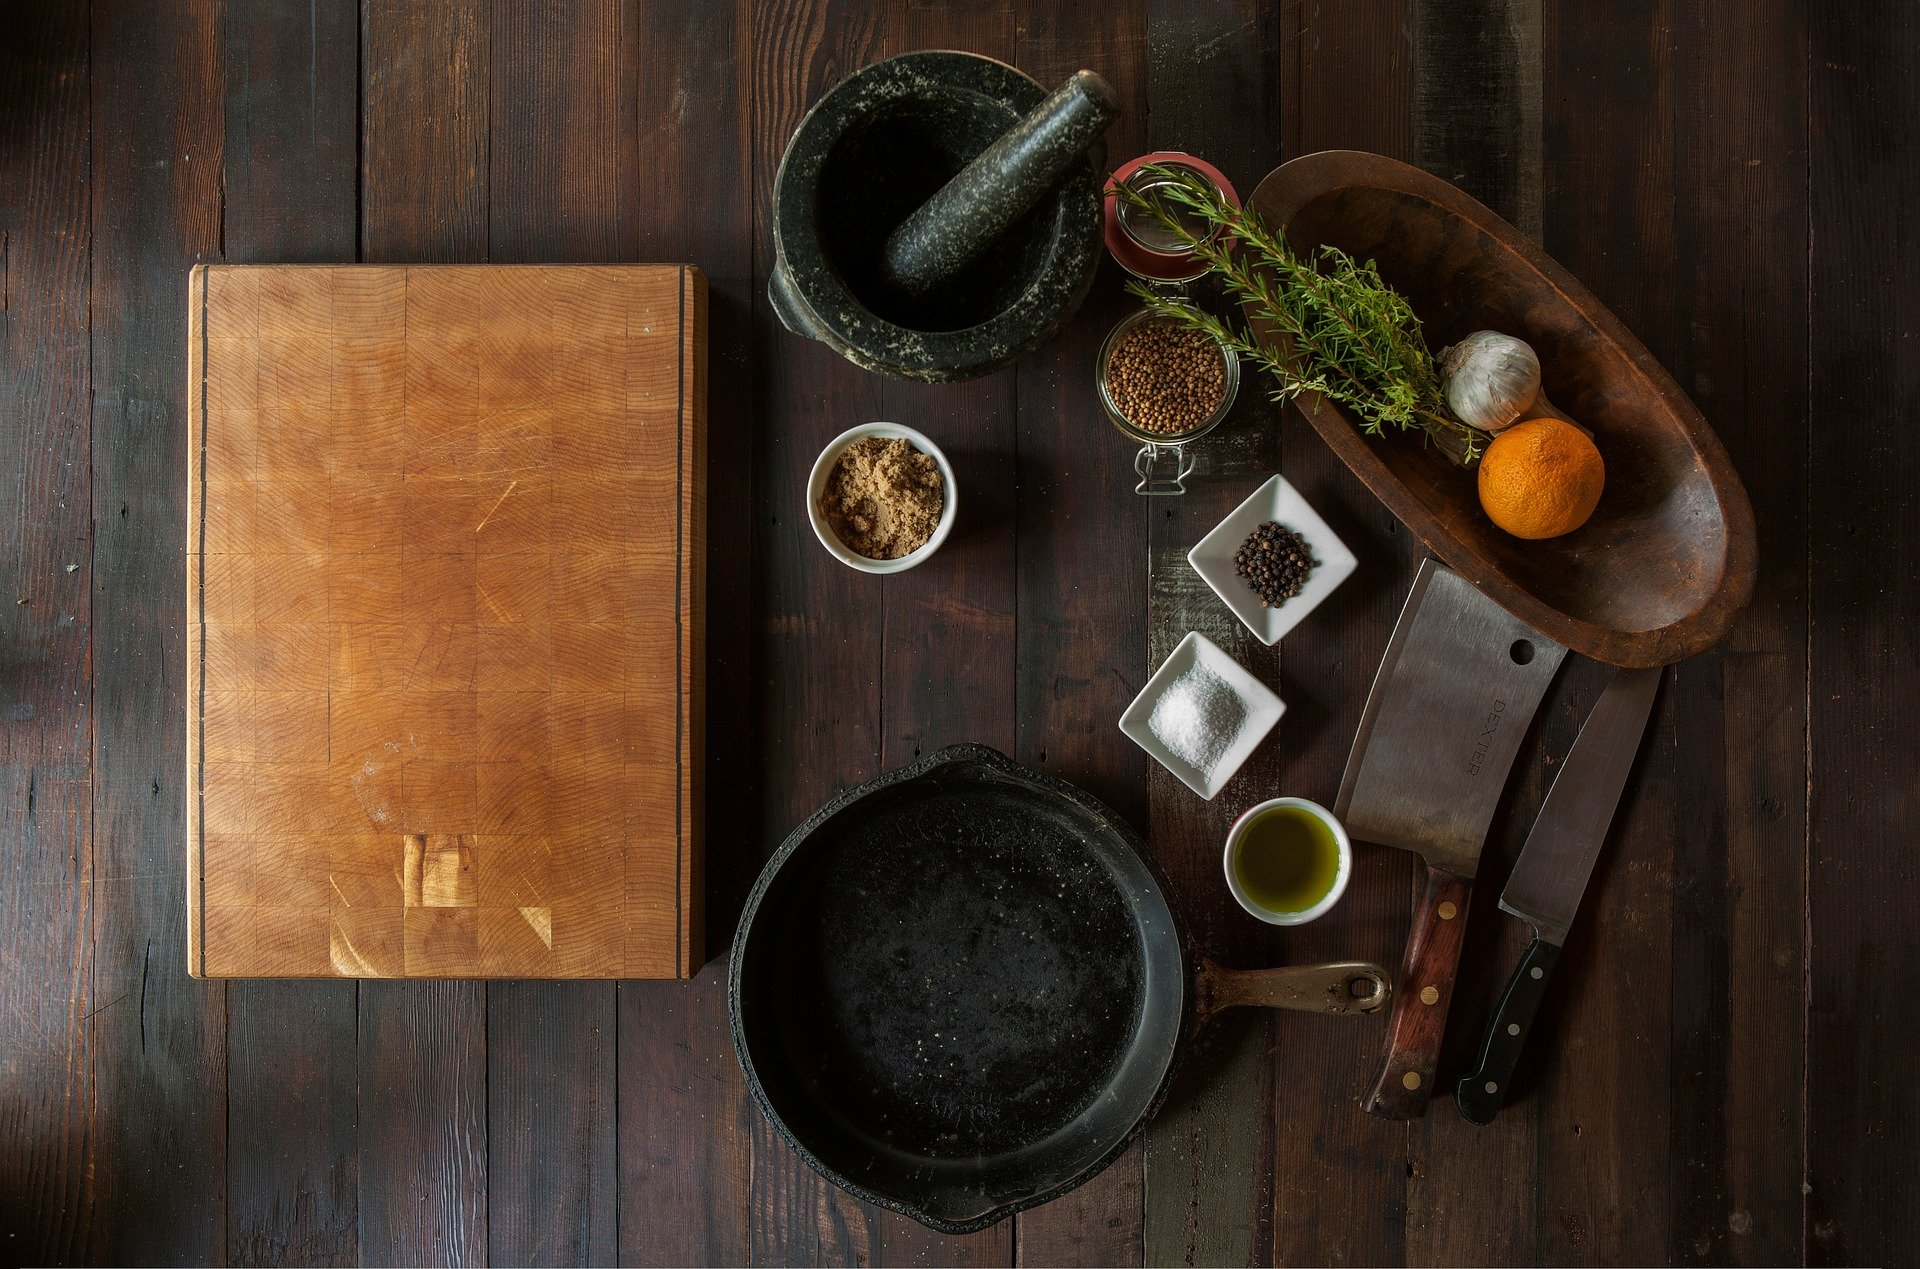
\includegraphics[scale=0.20]{images/ingredients-498199_1920.jpg}


\justify{}
Think of this chapter as the \emph{mise en place} of our DevSecOps souffle. We will increase our chances of success
by preparing our work environment for the project at hand. Let's start our preparations by outlining our
overall objectives. We want to:

\justify{}
\begin{itemize}
	\item
	      Create an extensible lab environment for rapid prototyping and development.
	\item
	      Keep our lab costs down while meeting the rest of the objectives.
	      Utilize free services and open source tools to the extent possible.
	\item
	      Use the published best practices for each tooling, operations, or
	      development ecosystem we choose to employ.
	\item
	      Always leave our projects in a functional state.
	\item
	      Get out of our old comfort zone, into a new one.
\end{itemize}

\section{Prerequisites}

\justify{}
This book intends to be a practical treatment of common and popular technologies from the DevSecOps world. As such, we assume
the reader has some basic knowledge of certain concepts. We will be exploring new ways of working for folks who
are somewhat familiar with:

\begin{itemize}
	\item
	    Linux (UI and command line)
	\item 
        Python 3
	\item
	    Familiarity with github.com and the concepts of pull requests and branching.
\end{itemize}

\justify{}
The examples in this book have been tested on Linux running the latest version of Docker. For more
intformation about installing Docker, see \href{https://docs.docker.com/get-docker/}{the Get Docker section}
of their website. There are directions there for installing Docker on Linux, Mac, and other operating systems.

Let's take a look at some of the other foundational environmental elements we need in place to be successful.

\section{Packages}

\subsection{MacOS}

Homebrew bills itself as \href{https://brew.sh/}{the missing package manager for MacOS}. Using ``brew'' and also
``cask'' to install and manage packages on MacOS will make your life much simpler.

\justify{}
It is also recommended that you familiarize yourself with the Terminal application on MacOS. Note that brew
commands are executed form within the terminal rather than using the GUI. Also bear in mind that packages are
installed with your user account. In other words, ``SuperUser'' privileges are not just discouraged, they are
neither required nor desired.

\subsection{Linux}

My prefered environment is a Debian based Linux distribution. Ubuntu, Cinnamon, and PopOS are all examples of 
Linux distrubutions in this family. While some code examples and lab containers use Debian-based distros, you
may also encounter Alpine Linux (typically chosen for it's smaller image size), amoung others.

\section{The Workhorse (IDE)}

\begin{figure}[!htb]
\centering
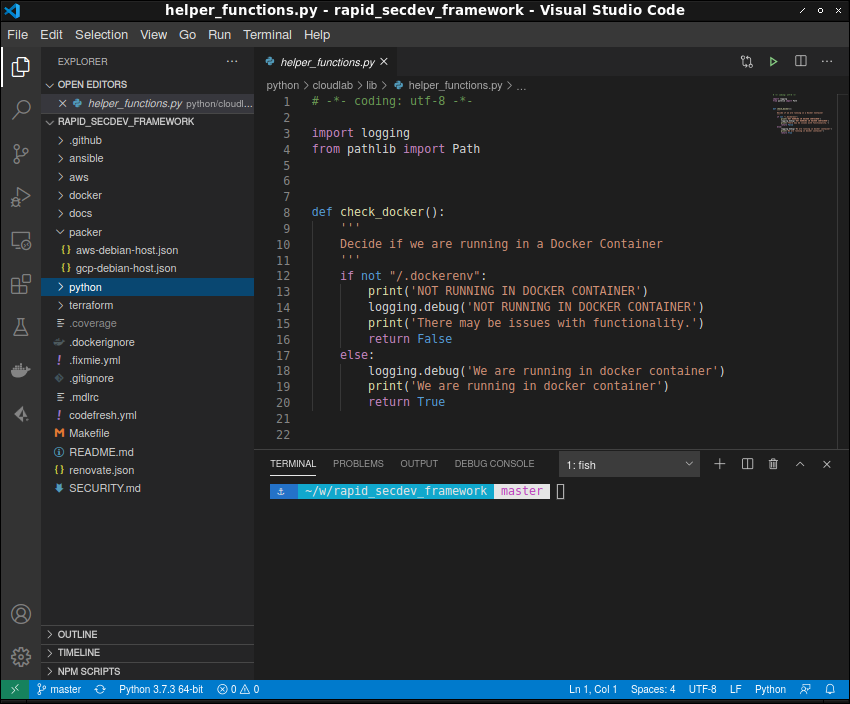
\includegraphics[scale=0.45]{images/setup-vscode.png}
\caption{The VScode IDE.}
\label{vscode-ide}
\end{figure}

\justify{}
It is quite helpful to have a piece of software on your workstation that makes code and document creation and edits easier. This
software is commonly known as an Integrated Development Environment (IDE)\index{IDE}. A decent IDE with the right add-ons can
provide syntax highlighting to show potential issues you might have missed, help you check for spelling or
grammar mistakes in your documentation, and even makes suggestions on alternate ways of writing your code.

\justify{}
There are many commercial and Open Source IDEs available. Visual Studio Code from Microsoft is a popular choice due to it's easy
installation. VSCode\index{VSCode} works well on Linux, Mac and other operating systems.
The environment is easily extensible to support most any language, linter, or syntax checker we may have a need
for, thanks to their easy to use and well integrated ``Extension'' feature. VSCode also has an integrated terminal
window\index{Terminal Window} so the developer can execute shell commands without leaving the IDE screen.

\section{SSH Key Setup}

\justify{}
Take note of the fact that setting up SSH keys means generating a pair of keys, not a single key. This is an important 
distinction. You will want to add your public key to sites like \href{github.com}{github.com}. The public key half will
also be added to machine instances that you create with public cloud providers. This will allow you to log in without
having to provision a user/password combination. You should take care to 
protect the private key at all times. Under no circumstances should you share your private SSH key.\cite{ssh}
\justify{}
Take a few minutes to generate an SSH key\index{SSH keys} pair if you don't already have one. We will add the public half of
our SSH key pair to hosts we provision. The directions for generating an SSH keypair found on the
\href{github.com}{github.com} website are perfect for our setup task. Follow the directions in the article 
\href{https://docs.github.com/en/github/authenticating-to-github/connecting-to-github-with-ssh/generating-a-new-ssh-key-and-adding-it-to-the-ssh-agent}{Generating a new SSH key and adding it to the ssh-agent}

\subsection{Generating a Key from the Command Line}

If you are using a Linux or Mac system, you have the option to create your SSH key pair from the command line. Consider 
the following example code listing.

\begin{mybox}{\thetcbcounter: SSH Key Generation}
\lstinputlisting{code/13-setup/ssh-key-generation}
\end{mybox}

\justify{}
Now you can add your public key half to your user settings in \href{github.com}{github.com}. For me it makes sense to have
two key pairs, one used for work projects, and one used for personal projects.

\section{GPG Key Setup}

\justify{}
\href{https://gnupg.org/}{Gnu Privacy Guard (GPG)} is an Open Source replacement for Symantec's PGP software. It allows you
to generate an asymmetric key pair that can be exchanged with other users, encrypt your personal files, or verify your identity.
Again, you will want to be sure to share your public key and protect your private key. This is the same reasoning we used in the
case of our SSH keys.

\justify{}
We will use a GPG key to sign commits to GitHub\index{GitHub}. This will help others verify that work you check in to revision
control did actually come from you. It's not strictly necessary but is considered good practice.
Some repositories require that you sign your pull requests with your GPG key\index{GPG key}.

\justify{}
Take a few minutes to set up a GPG key. Once you have an account setup, you can add
it to your profile on \href{github.com}{github.com}.

\subsection{Command Line GPG Key Setup}

\begin{mybox}{\thetcbcounter: Command Line GPG Key Setup}
\lstinputlisting{code/13-setup/gpg-key-setup}
\end{mybox}

\justify{}
Copy your GPG key, beginning with the string ``BEGIN PGP PUBLIC KEY BLOCK'' and ending with the string
``END PGP PUBLIC KEY BLOCK''. Add the GPG key to your GitHub account.

\section{Using pass to Encrypt Secrets Locally}

\justify{}
The pass program allows you to encrypt your keys, files, and other secrets in an encrypted database that is
stored in your home directory. Know that eventually, secrets leak. They can be exposed in a variety of ways, 
often they are committed to revision control by mistake.

\justify{}
Consider the following example where the pass program is used to encrypt secrets from a terminal window.

\begin{mybox}{\thetcbcounter: Encrypt Local Secrets on your Mac}
\lstinputlisting{code/13-setup/pass-mgr}
\end{mybox}

\section{Standard Project Layout}

\justify{}
The code examples in this book are organized in a standard way. The use of a known project 
layout across all project/repository directories increases the degree to which our projects can be used, reused, and
interoperate. Attention will be called to the folder and file naming conventions that are defined by this layout
as we encounter them.

\section{Installing Docker}

\justify{}
Recall that a properly functioning Docker setup on your local machine is a requirement for the upcoming
lab exercises. See the Docker website for 
\href{https://docs.docker.com/get-docker/}{instructions on how to install and configure Docker}. 

% include markdown file to populate a chapter with a lab from markdown files
\markdownInput{../labs/ch3/lab-3a.md}

\markdownInput{../labs/ch3/lab-3b.md}

\section{Directory Structure}

\justify{}
Relevant files and folders mentioned in this chapter are organized as seen below.

\begin{figure}[!htb]
	\centering
	\chapter{Getting Ready to Get Tactical}

\centering
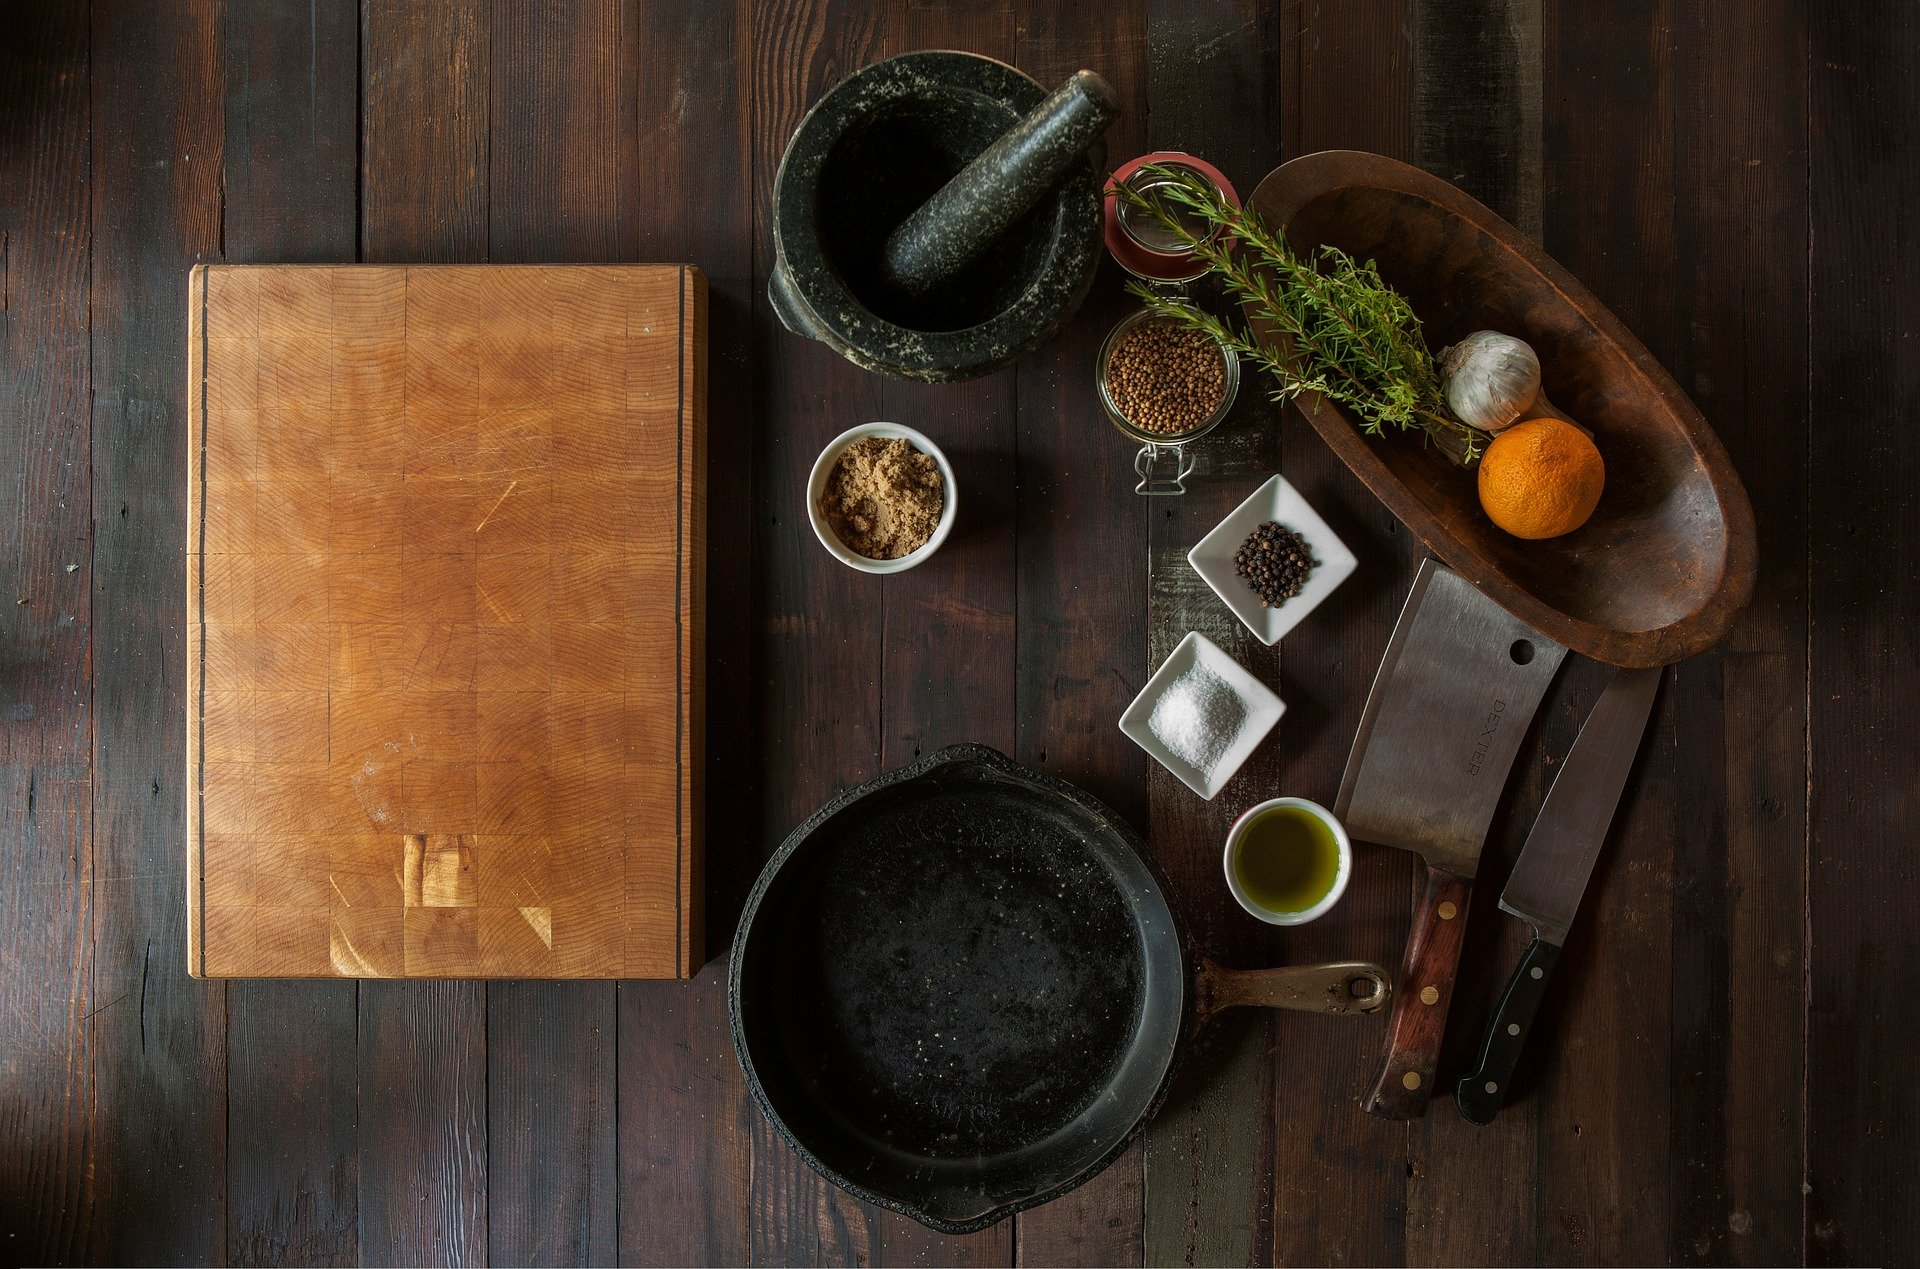
\includegraphics[scale=0.20]{images/ingredients-498199_1920.jpg}


\justify{}
Think of this chapter as the \emph{mise en place} of our DevSecOps souffle. We will increase our chances of success
by preparing our work environment for the project at hand. Let's start our preparations by outlining our
overall objectives. We want to:

\justify{}
\begin{itemize}
	\item
	      Create an extensible lab environment for rapid prototyping and development.
	\item
	      Keep our lab costs down while meeting the rest of the objectives.
	      Utilize free services and open source tools to the extent possible.
	\item
	      Use the published best practices for each tooling, operations, or
	      development ecosystem we choose to employ.
	\item
	      Always leave our projects in a functional state.
	\item
	      Get out of our old comfort zone, into a new one.
\end{itemize}

\section{Prerequisites}

\justify{}
This book intends to be a practical treatment of common and popular technologies from the DevSecOps world. As such, we assume
the reader has some basic knowledge of certain concepts. We will be exploring new ways of working for folks who
are somewhat familiar with:

\begin{itemize}
	\item
	    Linux (UI and command line)
	\item 
        Python 3
	\item
	    Familiarity with github.com and the concepts of pull requests and branching.
\end{itemize}

\justify{}
The examples in this book have been tested on Linux running the latest version of Docker. For more
intformation about installing Docker, see \href{https://docs.docker.com/get-docker/}{the Get Docker section}
of their website. There are directions there for installing Docker on Linux, Mac, and other operating systems.

Let's take a look at some of the other foundational environmental elements we need in place to be successful.

\section{Packages}

\subsection{MacOS}

Homebrew bills itself as \href{https://brew.sh/}{the missing package manager for MacOS}. Using ``brew'' and also
``cask'' to install and manage packages on MacOS will make your life much simpler.

\justify{}
It is also recommended that you familiarize yourself with the Terminal application on MacOS. Note that brew
commands are executed form within the terminal rather than using the GUI. Also bear in mind that packages are
installed with your user account. In other words, ``SuperUser'' privileges are not just discouraged, they are
neither required nor desired.

\subsection{Linux}

My prefered environment is a Debian based Linux distribution. Ubuntu, Cinnamon, and PopOS are all examples of 
Linux distrubutions in this family. While some code examples and lab containers use Debian-based distros, you
may also encounter Alpine Linux (typically chosen for it's smaller image size), amoung others.

\section{The Workhorse (IDE)}

\begin{figure}[!htb]
\centering
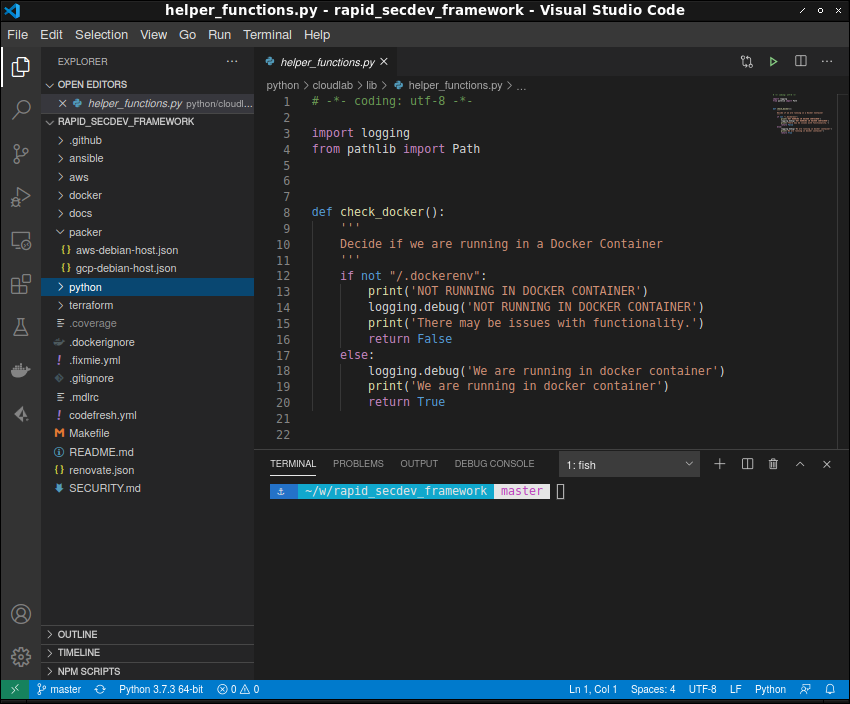
\includegraphics[scale=0.45]{images/setup-vscode.png}
\caption{The VScode IDE.}
\label{vscode-ide}
\end{figure}

\justify{}
It is quite helpful to have a piece of software on your workstation that makes code and document creation and edits easier. This
software is commonly known as an Integrated Development Environment (IDE)\index{IDE}. A decent IDE with the right add-ons can
provide syntax highlighting to show potential issues you might have missed, help you check for spelling or
grammar mistakes in your documentation, and even makes suggestions on alternate ways of writing your code.

\justify{}
There are many commercial and Open Source IDEs available. Visual Studio Code from Microsoft is a popular choice due to it's easy
installation. VSCode\index{VSCode} works well on Linux, Mac and other operating systems.
The environment is easily extensible to support most any language, linter, or syntax checker we may have a need
for, thanks to their easy to use and well integrated ``Extension'' feature. VSCode also has an integrated terminal
window\index{Terminal Window} so the developer can execute shell commands without leaving the IDE screen.

\section{SSH Key Setup}

\justify{}
Take note of the fact that setting up SSH keys means generating a pair of keys, not a single key. This is an important 
distinction. You will want to add your public key to sites like \href{github.com}{github.com}. The public key half will
also be added to machine instances that you create with public cloud providers. This will allow you to log in without
having to provision a user/password combination. You should take care to 
protect the private key at all times. Under no circumstances should you share your private SSH key.\cite{ssh}
\justify{}
Take a few minutes to generate an SSH key\index{SSH keys} pair if you don't already have one. We will add the public half of
our SSH key pair to hosts we provision. The directions for generating an SSH keypair found on the
\href{github.com}{github.com} website are perfect for our setup task. Follow the directions in the article 
\href{https://docs.github.com/en/github/authenticating-to-github/connecting-to-github-with-ssh/generating-a-new-ssh-key-and-adding-it-to-the-ssh-agent}{Generating a new SSH key and adding it to the ssh-agent}

\subsection{Generating a Key from the Command Line}

If you are using a Linux or Mac system, you have the option to create your SSH key pair from the command line. Consider 
the following example code listing.

\begin{mybox}{\thetcbcounter: SSH Key Generation}
\lstinputlisting{code/13-setup/ssh-key-generation}
\end{mybox}

\justify{}
Now you can add your public key half to your user settings in \href{github.com}{github.com}. For me it makes sense to have
two key pairs, one used for work projects, and one used for personal projects.

\section{GPG Key Setup}

\justify{}
\href{https://gnupg.org/}{Gnu Privacy Guard (GPG)} is an Open Source replacement for Symantec's PGP software. It allows you
to generate an asymmetric key pair that can be exchanged with other users, encrypt your personal files, or verify your identity.
Again, you will want to be sure to share your public key and protect your private key. This is the same reasoning we used in the
case of our SSH keys.

\justify{}
We will use a GPG key to sign commits to GitHub\index{GitHub}. This will help others verify that work you check in to revision
control did actually come from you. It's not strictly necessary but is considered good practice.
Some repositories require that you sign your pull requests with your GPG key\index{GPG key}.

\justify{}
Take a few minutes to set up a GPG key. Once you have an account setup, you can add
it to your profile on \href{github.com}{github.com}.

\subsection{Command Line GPG Key Setup}

\begin{mybox}{\thetcbcounter: Command Line GPG Key Setup}
\lstinputlisting{code/13-setup/gpg-key-setup}
\end{mybox}

\justify{}
Copy your GPG key, beginning with the string ``BEGIN PGP PUBLIC KEY BLOCK'' and ending with the string
``END PGP PUBLIC KEY BLOCK''. Add the GPG key to your GitHub account.

\section{Using pass to Encrypt Secrets Locally}

\justify{}
The pass program allows you to encrypt your keys, files, and other secrets in an encrypted database that is
stored in your home directory. Know that eventually, secrets leak. They can be exposed in a variety of ways, 
often they are committed to revision control by mistake.

\justify{}
Consider the following example where the pass program is used to encrypt secrets from a terminal window.

\begin{mybox}{\thetcbcounter: Encrypt Local Secrets on your Mac}
\lstinputlisting{code/13-setup/pass-mgr}
\end{mybox}

\section{Standard Project Layout}

\justify{}
The code examples in this book are organized in a standard way. The use of a known project 
layout across all project/repository directories increases the degree to which our projects can be used, reused, and
interoperate. Attention will be called to the folder and file naming conventions that are defined by this layout
as we encounter them.

\section{Installing Docker}

\justify{}
Recall that a properly functioning Docker setup on your local machine is a requirement for the upcoming
lab exercises. See the Docker website for 
\href{https://docs.docker.com/get-docker/}{instructions on how to install and configure Docker}. 

% include markdown file to populate a chapter with a lab from markdown files
\markdownInput{../labs/ch3/lab-3a.md}

\markdownInput{../labs/ch3/lab-3b.md}

\section{Directory Structure}

\justify{}
Relevant files and folders mentioned in this chapter are organized as seen below.

\begin{figure}[!htb]
	\centering
	\chapter{Getting Ready to Get Tactical}

\centering
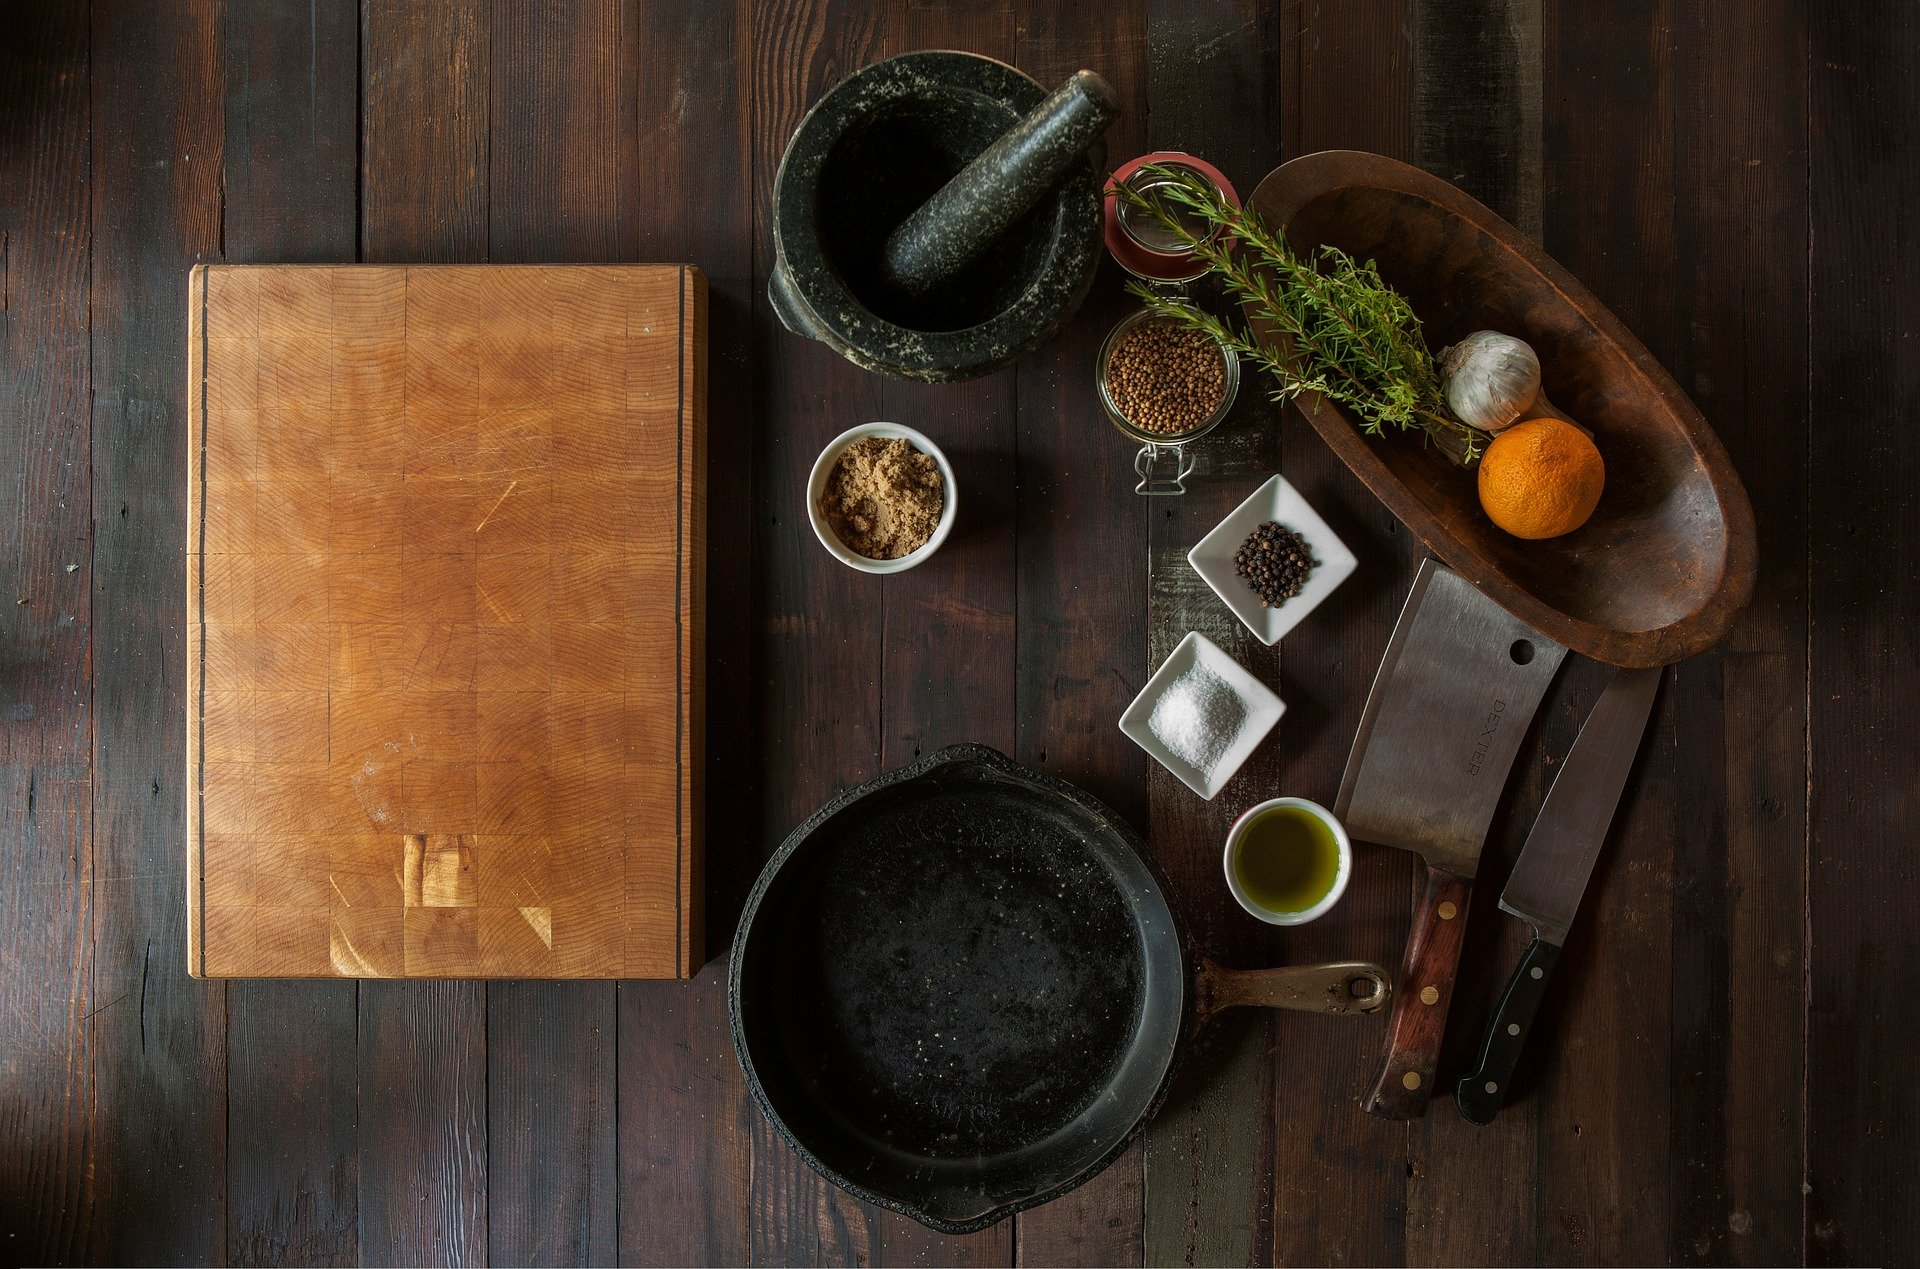
\includegraphics[scale=0.20]{images/ingredients-498199_1920.jpg}


\justify{}
Think of this chapter as the \emph{mise en place} of our DevSecOps souffle. We will increase our chances of success
by preparing our work environment for the project at hand. Let's start our preparations by outlining our
overall objectives. We want to:

\justify{}
\begin{itemize}
	\item
	      Create an extensible lab environment for rapid prototyping and development.
	\item
	      Keep our lab costs down while meeting the rest of the objectives.
	      Utilize free services and open source tools to the extent possible.
	\item
	      Use the published best practices for each tooling, operations, or
	      development ecosystem we choose to employ.
	\item
	      Always leave our projects in a functional state.
	\item
	      Get out of our old comfort zone, into a new one.
\end{itemize}

\section{Prerequisites}

\justify{}
This book intends to be a practical treatment of common and popular technologies from the DevSecOps world. As such, we assume
the reader has some basic knowledge of certain concepts. We will be exploring new ways of working for folks who
are somewhat familiar with:

\begin{itemize}
	\item
	    Linux (UI and command line)
	\item 
        Python 3
	\item
	    Familiarity with github.com and the concepts of pull requests and branching.
\end{itemize}

\justify{}
The examples in this book have been tested on Linux running the latest version of Docker. For more
intformation about installing Docker, see \href{https://docs.docker.com/get-docker/}{the Get Docker section}
of their website. There are directions there for installing Docker on Linux, Mac, and other operating systems.

Let's take a look at some of the other foundational environmental elements we need in place to be successful.

\section{Packages}

\subsection{MacOS}

Homebrew bills itself as \href{https://brew.sh/}{the missing package manager for MacOS}. Using ``brew'' and also
``cask'' to install and manage packages on MacOS will make your life much simpler.

\justify{}
It is also recommended that you familiarize yourself with the Terminal application on MacOS. Note that brew
commands are executed form within the terminal rather than using the GUI. Also bear in mind that packages are
installed with your user account. In other words, ``SuperUser'' privileges are not just discouraged, they are
neither required nor desired.

\subsection{Linux}

My prefered environment is a Debian based Linux distribution. Ubuntu, Cinnamon, and PopOS are all examples of 
Linux distrubutions in this family. While some code examples and lab containers use Debian-based distros, you
may also encounter Alpine Linux (typically chosen for it's smaller image size), amoung others.

\section{The Workhorse (IDE)}

\begin{figure}[!htb]
\centering
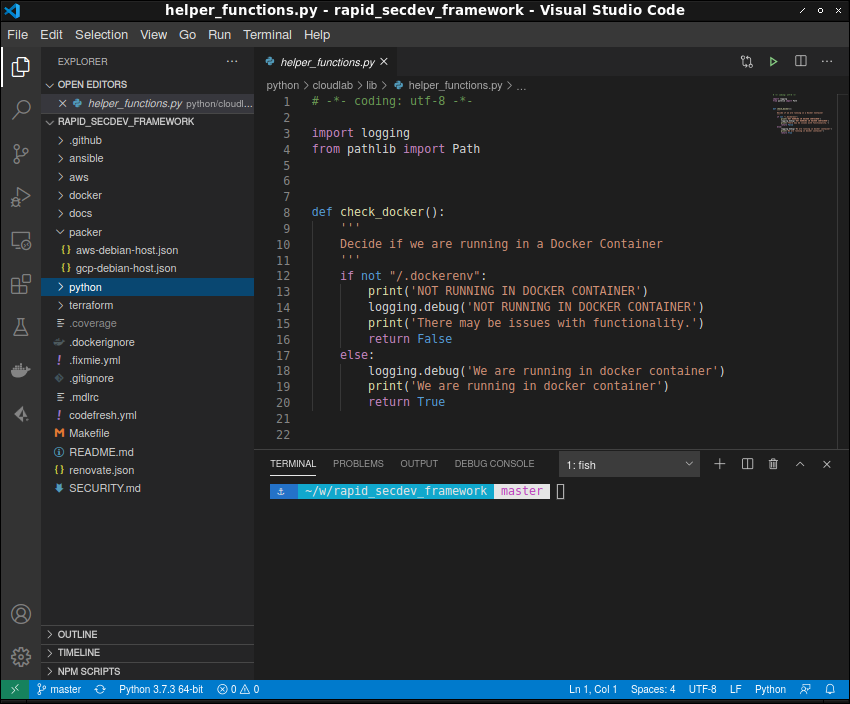
\includegraphics[scale=0.45]{images/setup-vscode.png}
\caption{The VScode IDE.}
\label{vscode-ide}
\end{figure}

\justify{}
It is quite helpful to have a piece of software on your workstation that makes code and document creation and edits easier. This
software is commonly known as an Integrated Development Environment (IDE)\index{IDE}. A decent IDE with the right add-ons can
provide syntax highlighting to show potential issues you might have missed, help you check for spelling or
grammar mistakes in your documentation, and even makes suggestions on alternate ways of writing your code.

\justify{}
There are many commercial and Open Source IDEs available. Visual Studio Code from Microsoft is a popular choice due to it's easy
installation. VSCode\index{VSCode} works well on Linux, Mac and other operating systems.
The environment is easily extensible to support most any language, linter, or syntax checker we may have a need
for, thanks to their easy to use and well integrated ``Extension'' feature. VSCode also has an integrated terminal
window\index{Terminal Window} so the developer can execute shell commands without leaving the IDE screen.

\section{SSH Key Setup}

\justify{}
Take note of the fact that setting up SSH keys means generating a pair of keys, not a single key. This is an important 
distinction. You will want to add your public key to sites like \href{github.com}{github.com}. The public key half will
also be added to machine instances that you create with public cloud providers. This will allow you to log in without
having to provision a user/password combination. You should take care to 
protect the private key at all times. Under no circumstances should you share your private SSH key.\cite{ssh}
\justify{}
Take a few minutes to generate an SSH key\index{SSH keys} pair if you don't already have one. We will add the public half of
our SSH key pair to hosts we provision. The directions for generating an SSH keypair found on the
\href{github.com}{github.com} website are perfect for our setup task. Follow the directions in the article 
\href{https://docs.github.com/en/github/authenticating-to-github/connecting-to-github-with-ssh/generating-a-new-ssh-key-and-adding-it-to-the-ssh-agent}{Generating a new SSH key and adding it to the ssh-agent}

\subsection{Generating a Key from the Command Line}

If you are using a Linux or Mac system, you have the option to create your SSH key pair from the command line. Consider 
the following example code listing.

\begin{mybox}{\thetcbcounter: SSH Key Generation}
\lstinputlisting{code/13-setup/ssh-key-generation}
\end{mybox}

\justify{}
Now you can add your public key half to your user settings in \href{github.com}{github.com}. For me it makes sense to have
two key pairs, one used for work projects, and one used for personal projects.

\section{GPG Key Setup}

\justify{}
\href{https://gnupg.org/}{Gnu Privacy Guard (GPG)} is an Open Source replacement for Symantec's PGP software. It allows you
to generate an asymmetric key pair that can be exchanged with other users, encrypt your personal files, or verify your identity.
Again, you will want to be sure to share your public key and protect your private key. This is the same reasoning we used in the
case of our SSH keys.

\justify{}
We will use a GPG key to sign commits to GitHub\index{GitHub}. This will help others verify that work you check in to revision
control did actually come from you. It's not strictly necessary but is considered good practice.
Some repositories require that you sign your pull requests with your GPG key\index{GPG key}.

\justify{}
Take a few minutes to set up a GPG key. Once you have an account setup, you can add
it to your profile on \href{github.com}{github.com}.

\subsection{Command Line GPG Key Setup}

\begin{mybox}{\thetcbcounter: Command Line GPG Key Setup}
\lstinputlisting{code/13-setup/gpg-key-setup}
\end{mybox}

\justify{}
Copy your GPG key, beginning with the string ``BEGIN PGP PUBLIC KEY BLOCK'' and ending with the string
``END PGP PUBLIC KEY BLOCK''. Add the GPG key to your GitHub account.

\section{Using pass to Encrypt Secrets Locally}

\justify{}
The pass program allows you to encrypt your keys, files, and other secrets in an encrypted database that is
stored in your home directory. Know that eventually, secrets leak. They can be exposed in a variety of ways, 
often they are committed to revision control by mistake.

\justify{}
Consider the following example where the pass program is used to encrypt secrets from a terminal window.

\begin{mybox}{\thetcbcounter: Encrypt Local Secrets on your Mac}
\lstinputlisting{code/13-setup/pass-mgr}
\end{mybox}

\section{Standard Project Layout}

\justify{}
The code examples in this book are organized in a standard way. The use of a known project 
layout across all project/repository directories increases the degree to which our projects can be used, reused, and
interoperate. Attention will be called to the folder and file naming conventions that are defined by this layout
as we encounter them.

\section{Installing Docker}

\justify{}
Recall that a properly functioning Docker setup on your local machine is a requirement for the upcoming
lab exercises. See the Docker website for 
\href{https://docs.docker.com/get-docker/}{instructions on how to install and configure Docker}. 

% include markdown file to populate a chapter with a lab from markdown files
\markdownInput{../labs/ch3/lab-3a.md}

\markdownInput{../labs/ch3/lab-3b.md}

\section{Directory Structure}

\justify{}
Relevant files and folders mentioned in this chapter are organized as seen below.

\begin{figure}[!htb]
	\centering
	\input{dot/13-setup.tex}
	\caption{Setup related files.}
	\label{setupfiles}
\end{figure}


	\caption{Setup related files.}
	\label{setupfiles}
\end{figure}


	\caption{Setup related files.}
	\label{setupfiles}
\end{figure}


	\caption{Setup related files.}
	\label{setupfiles}
\end{figure}

